% !TEX root = ../main.tex

\chapter{Technical development} % (fold)
\label{chp:execution}

\section{Terminology}
\label{sec:terminology}

The Algolia API is pushing by uploading schemaless \acrshort{json} Objects to an index %%

\section{Organizing state} % (fold)
\label{sec:organizing_state}

\subsection{Widgets and connectors}
\label{sub:widgets_and_connectors}

The big difference between using Algolia with the Helper compared to InstantSearch is the notion of widgets. In the current implementations there are ten core widgets. Each of these widgets is split up in its logic (a connector) and its display logic (a component). Together these widgets are:

\begin{itemize}
  \item SearchBox
  \item Hits
  \item RefinementList
  \item Range
  \item Pagination
  \item ClearAll
  \item CurrentRefinements
  \item Sort By
  \item Highlight
  \item Snippet
\end{itemize}

There are two kinds of widgets, interactive widgets and display-only widgets. Display-only widgets read the current results and applied \glspl{refinement} from the Algolia response. The display-only widgets are Hits, which is a representation of all the results. The other two are Highlight and Snippet, which take an attribute, and display the snipped and highlighted result from the Algolia response.

The other widgets are interactive widgets. They also take their display value from the response, to show which facets are enabled, or which \gls{refinement} is already made. All of them also expose a {\tt refine()} function. This function will be called whenever is applicable in that case, and uses Helper methods like {\tt helper.state.toggleRefinement} to actually apply their change on the search state.

%% talk about the difference between storing parameters and storing widget state

\subsection{Structuring a state container}
\label{sub:structuring_a_state_container}

In the InstantSearch Core implementation the choice has been made to structure state in three divisions. One for the result that comes from each API call, one for raw parameters like {\tt DISTINCT} and another division for the actual \glspl{refinement}.

Since InstantSearch Core is a JavaScript \gls{library}, there is not much choice for a container. A {\tt Map}\cite{mdn-map} could be used as the actual value for the {\tt result} key, but since it's not widely supported and has a significantly less elegant API, and they generally consume more memory in smaller Objects. Since in the general case, Algolia results contain about 20 hits, and a finite amount of filters, using {\tt Object} is perfectly reasonable.

\begin{minipage}{\linewidth}
\begin{lstlisting}[caption={The state container of InstantSearch Core},label={lst:is-core-state-1}]
const state = {
  refinements,
  rawParameters,
  result,
};
\end{lstlisting}
\end{minipage}

Here, the most interesting container is the {\tt refinement} container. It's structured as another {\tt Object} with a key for every \gls{attribute} name which is being refined, and is inspired by the structure of the state {\tt Object} in React InstantSearch\cite{react-instantsearch-search-state}.

Every \gls{attribute} is another {\tt Object}, with a {\tt type} key, and a {\tt value} key. For each of the possible \glspl{refinement}, a value that is relevant is chosen. 

A menu for example is a \gls{refinement} that takes a \gls{attribute} that has been set up for faceting\cite{algolia-set-up-faceting} and has a single value. For that reason a menu takes in a string as a value. A list is a \gls{refinement} that is exactly the same, but takes a list of strings to be able to set up multiple refined values for that attribute.

Having a structure like this implies that it is trivial to see if any \glspl{refinement} have been set, including the query. This is useful for when an interface is constructed that only shows a search bar until the first character is typed. After that a more elaborate interface shows up to fill the screen with other filters.

If every refinement would be set, the \glspl{refinement} key of the search state would be:

\begin{minipage}{\linewidth}
\begin{lstlisting}[caption={\Glspl{refinement} in InstantSearch Core},label={lst:is-core-state-2}]
const refinements = {
  color: {
    type: 'menu',
    value: 'blue',
  },
  products: {
    type: 'hierarchicalMenu',
    value: 'Laptops > Surface',
  },
  brand: {
    type: 'list',
    value: ['apple', 'samsung'],
  },
  price: {
    type: 'range',
    value: {
      min: 20,
      max: 3000
    },
  },
  freeShipping: {
    type: 'toggle',
    value: false,
  },
  query: {
    type: 'query',
    value: 'pizza',
  },
  page: {
    type: 'page',
    value: 1,
  },
};
\end{lstlisting}
\end{minipage}

To be able to handle a lot of cases that can't be foreseen by the \glspl{refinement}, or to handle settings that aren't visible to the user, a {\tt rawParameters} key is available in the search state. 

These \gls{attribute} names will be used in the results, exactly as they are in the query, and always supersede the \glspl{refinement}, since usually when someone needs custom parameters that aren't provided by a refinement, they have a good reason for that.

\begin{minipage}{\linewidth}
\begin{lstlisting}[caption={Passing raw Algolia parameters to InstantSearch Core},label={lst:is-core-state-3}]
const rawParameters = {
  distinct: true,
  page: 3,
};
\end{lstlisting}
\end{minipage}

Finally, and maybe more importantly are the results. The results are not exactly the same as how they come in from the Algolia API. The differentiator is that there is a slight reordering to match the structure of the {\tt refinement} block.

This solves an interesting problem with InstantSearch.js. Whenever something needs to be done which isn't provided by the \gls{library}, a so-called custom widget needs to be written. To be able to call any Algolia related functionality, the Helper is used. 

When certain functionality is needed, there's a gap in terminology between the widgets and the actual Algolia parameters. For example: what's called a menu widget in InstantSearch.js, is called a hierarchicalRefinement. In most cases this doesn't really matter, but when someone needs to recreate a widget without a connector, they should know that the terminology can be different.

\begin{minipage}{\linewidth}
\begin{lstlisting}[caption={Results container in the InstantSearch Core state},label={lst:is-core-state-4}]
const result = {
  color: {
    type: 'menu',
    value: [
      {
        label: 'red',
        count: 10,
      },
      {
        label: 'blue',
        count: 100,
      },
    ],
  },
  (*@{\vdots}@*)
  hits: [
    {
      ObjectID: '0x1f355',
      color: 'blue',
     (*@{\vdots}@*)
    },
    (*@{\vdots}@*)
  ],
  meta: { 
    processingTimeMS: 5,
    (*@{\vdots}@*)
  },
};
\end{lstlisting}
\end{minipage}

Because of this structure, a connector can be made for every refinement. It will change something in a refinement, and subscribe for the changes to the results, and only needs to take one key into account. Ultimately this leads to a more understandable API for people using this \gls{library}.

This state container is called {\tt InstantSearch}, because it's meant to be used in both InstantSearch.js, React InstantSearch, the upcoming Vue InstantSearch, as well as other community versions of InstantSearch, see also section \ref{sec:usage_in_libraries} for a more complete study on that.

% section organizing_state (end)

\section{Handling state changes} % (fold)
\label{sec:handling_state_changes}

\subsection{InstantSearch}
\label{ssec:instantsearch}

The InstantSearch state container is exposed as a factory function creating a new container. The {\tt createInstantSearch} function inherits from the {\tt createStore} function used in other parts of the \gls{library}, see figure \ref{figure:createstore_inheritance} for the complete architecture. It allows to be subscribed to with a function as argument that will be called each time a change happens to the state, with the new state as arguments.

While all three keys of the state container will change over time, they each work in a slightly different way. The {\tt results} key is described in section \ref{sec:getting_responses_from_the_api}, and is tracked fairly straightforward. Every time a new API response comes in, it will completely overwrite the previous state of that key. 

\subsection{Raw \glspl{refinement}}
\label{ssec:raw-refinments}

All raw parameters are being rewritten in place, similar to how {\tt setState} works in React~\cite{react-doc-state}~. A function called {\tt refineRaw} is exposed on a state container. This function expects a function as an argument. It receives the previous state for the \glspl{refinement} as its parameter, and is expected to return the new state Object, based on whatever happened that needs to change.

This pattern allows a developer to have the freedom to change whatever parameters are necessary to change, while having access to the complete truth at that point easily. An example of toggling the {\tt DISTINCT} parameter, for example on an event listener for a button with that purpose would look like this:

\begin{minipage}{\linewidth}
\begin{lstlisting}[caption={Toggling the {\tt DISTINCT} parameter},label={lst:is-core-raw}]
function toggleDistinct(previousState) {
  // set the distinct parameter as the opposite of previously
  const oppositeDistinct = { distinct: !previousState.distinct };

  // make an Object to hold the new state
  const newState = Object.assign({}, previousState, oppositeDistinct);
  return newState;
}

state.refineRaw(toggleDistinct);
\end{lstlisting}
\end{minipage}

In future JavaScript engines\footnote{spread properties on Objects are currently a Stage 3 proposal for \acrshort{ecmascript}\cite{es-prop-spread}, which means they are starting to be implemented by browsers, but it isn't part of the standard yet.}, it will be able to write this kind of code using spread properties on Objects. This kind of pattern would look like this then:

\begin{minipage}{\linewidth}
\begin{lstlisting}[caption={Toggling the {\tt DISTINCT} parameter when Object spread is available},label={lst:is-core-raw-es2015}]
function toggleDistinct(previousState) {
  return {
    ...previousState,
    distinct: distinct: !previousState.distinct,
  }
}

state.refineRaw(toggleDistinct);
\end{lstlisting}
\end{minipage}

\subsection{Refinements}
\label{ssec:refinments}

The complete state container is structured in the same way as a single refinement. It's a factory function, returning an Object. This Object has three functions: 

\begin{enumerate}
  \item {\tt get state()}
  \item {\tt subscribe()}
  \item {\tt setState()} or {\tt refine()}
\end{enumerate}

A basic {\tt store}

\begin{figure}[H]
  \centering
  \includegraphics[width=.5\textwidth, draft]{../assets/createStore.pdf}
  \caption{InstantSearch Core store organisation.}
  \label{figure:createstore_inheritance}
\end{figure}

\subsection{Subscribing}
\label{ssec:Subscribing}

The big differentiator between some of the big frontend frameworks nowadays is how they handle state changes. To make sure that InstantSearch Core to be used in all major methodologies, three different interfaces are exposed.

\subsubsection{Getters}
\label{ssub:getters}

While at any moment it's possible to call the state getter on an InstantSearch store or a refinement, a programmer might want to know how state changes overtime, and get notified about the new change. If only the state getter would be implemented, a naive way to find out about changes, is repeatedly asking for the current state like this:

\begin{minipage}{\linewidth}
\begin{lstlisting}[caption={Naive way to find out about changed state},label={lst:is-core-naive-subscribe}]
// holder for the state
let currentState = {};

function update() {
  // reassign the state
  currentState = store.state;
  requestAnimationFrame(update);
}

// call the update function when a new frame is being drawn
requestAnimationFrame(update);
\end{lstlisting}
\end{minipage}

After that, the {\tt currentState} variable might be used wherever it's needed, and make the needed UI changes. Depending on the type of framework used for this, it might either have a very big impact, or be optimised away, but it isn't always ideal.

For a framework like Vue\cite{vue-reactivity}, this approach is close to the way to go. There is no implicit need for reassigning a local variable, since the {\tt store} is available with a getter. Vue will track the changes to all getters on Objects with a process called ``reactive values''.

Vue will trigger a new render on every frame where there has been time for it, which gives it the time to call a getter function on every frame seamlessly. 

\subsubsection{Subscribe function}
\label{ssub:subscribe_function}

Not all frameworks implement this kind of reactivity. React for example will only look at the \gls{props} and context of a component. It would be possible to pass down the {\tt store.state} getter as part of React context, but it would cause unneeded renders, since that part of optimisation is left over to the user land of a React app. 

For frameworks like React, a {\tt subscribe()} function is available at the store prototype. Similar to Redux\cite{redux-glossary-store}, a state management \gls{library} that works very well with React, this function expects a single function as the argument. This function will be called at every time the state changes, be it either by changing \glspl{refinement}, or by new results being returned.

%% say that you then pass that data through using props or context

\subsubsection{Observables}
\label{ssub:observables}

An upcoming proposed standard for \acrshort{ecmascript} is observables.The \acrshort{ecmascript} proposal for Observables is currently stage 0\cite{tc39-observable}, that means that it will not be part of JavaScript until it has been voted for, and went through the process. It's currently not implemented in any browser without libraries. These Observables signify a variable that will change over time, and that will let its subscribers know about the changes.

This pattern is very close to previous method, subscriptions, but then as part of the language, and not a decided upon standard. Using language features has the advantage that over time more libraries will use this pattern and it will make the API surface of the \gls{library} smaller.

Since the observables implementation in JavaScript is a proposal, a reference implementation has been made by zenparsing, the author of the proposal. The \gls{library} called {\tt zen-observable}\cite{zenparsing-observable} is extending the API of the Observable proposal slightly, but in its core, it has the same concepts.

An instance of an Observable is returned from the store interface, by using the {\tt symbol-observable}\cite{symbol-observable} ponyfill module. A ponyfill\cite{ponyfill} is a module with the functionality of an upcoming language API, made with the current capabilities of the platform. The difference between a polyfill and a ponyfill is that a polyfill will overwrite the implementation of the API if it is implemented in browsers, while a ponyfill intentionally uses a slightly different name.

Just like in the previous section, an Observable will expose a subscribe function. The difference here is that it expects to be subscribed with an Object. This Object contains three functions, that are called when respectively the {\tt next}, {\tt error} or {\tt complete} event have been called by the observable.

Having a interoperability layer with observables means that InstantSearch means that it will work well with the frameworks that use observables as a core of their infrastructure. Angular is an example of a framework that has observables --- in the form of RxJS\cite{angular-rx} --- as an important part of its way to work with events.


% section handling_state_changes (end)

\section{Getting responses from the API} % (fold)
\label{sec:getting_responses_from_the_api}

another function listens to changes in state %%

it transforms params into a JS client request

it replaces the {\tt response} in the state with an action

% section getting_responses_from_the_api (end)

\section{Rendering \glspl{refinement}} % (fold)
\label{sec:rendering_refinements}

When using InstantSearch to render refinement in a widget or a connector, it comes down to three distinct steps:

\begin{enumerate}
  \item create the refinement
  \item update the relevant \acrshort{dom} with the data from Algolia
  \item send \glspl{refinement} when certain events are triggered
\end{enumerate}

The things that need to happen here are almost exactly what needs to happen when making a connector using InstantSearch.js. React InstantSearch is more of an exception here, since it uses the functional composition of connector functions.

In regular JavaScript, these paradigms could go over the heads of normal developers, which is why the choice to leave the two definitions of connectors.

\subsection{Creating a refinement}
\label{subs:creating_a_refinement}

To create a refinement, two steps happen. Firstly a new refinement container is created. This has a very similar structure as described in section \ref{ssec:refinments}. The next step is to register that refinement to the InstantSearch store.

As an example, a refinement list is created from the ``brands'' attribute. %%

\begin{minipage}{\linewidth}
\begin{lstlisting}[caption={Creating a refinement},label={lst:creating-refinement}]
import { createRefinementlist } from 'instantsearch-core/refinements';

const brands = createRange({attributeName: 'brands'});

export default brands;
\end{lstlisting}
\end{minipage}

blimbo: do it cool and register %%

\begin{minipage}{\linewidth}
\begin{lstlisting}[caption={Registering a refinement},label={lst:registering-refinement}]
import { store } 
\end{lstlisting}
\end{minipage}

\subsection{Updating or creating \acrshort{dom} with Algolia data}
\label{subs:data_to_dom}

Simple dom making yo %%

\subsection{Calling the {\tt refine} function}
\label{subs:refining}

yo press the button and update the dom %%

% section rendering_\glspl{refinement} (end)

\section{Saved state} % (fold)
\label{sec:saved_state}

The API also allows for an initialisation with a certain state passed in. This means that it's possible to save a state Object in a location, and then later restart the search from that data. 

This is useful for three major use cases. The first is \acrshort{url} synchronisation. For \acrshort{url} synchronisation the structure would be to first listen on every state change with {\tt .subscribe()}, and then asynchronously transform that to query parameters to set. If a user comes to a page with query parameters, a function to take in the query string and put out a state Object would then be called. After that point a new InstantSearch Core instance can be built with the {\tt preloadedState} parameter set in the constructor.

\begin{figure}[H]
  \centering
  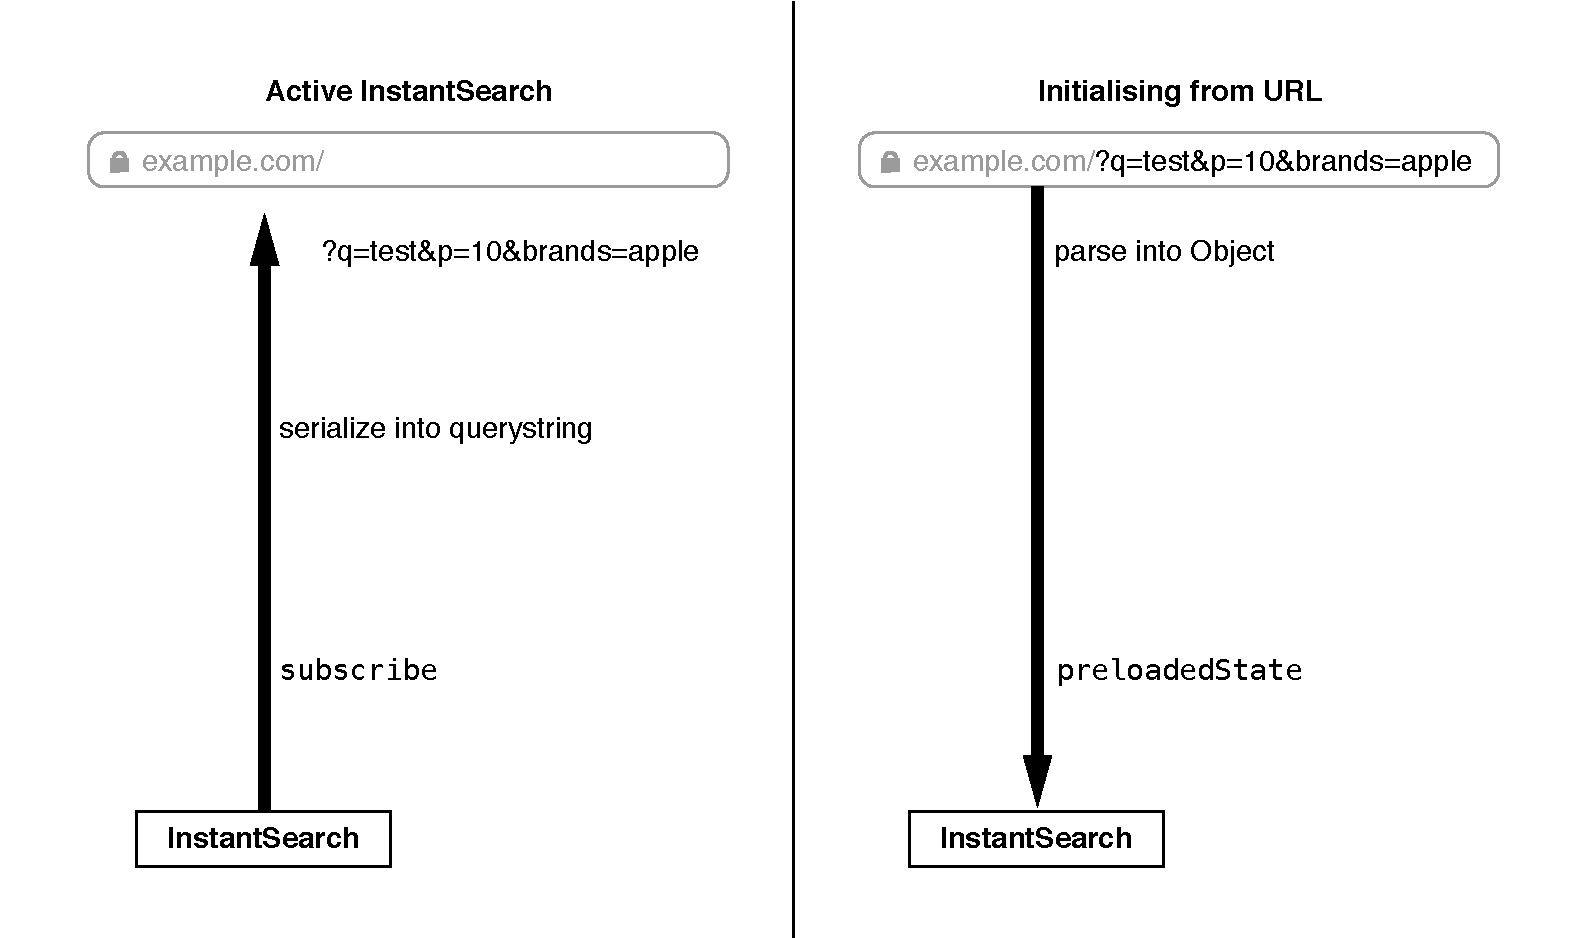
\includegraphics[width=0.6\textwidth, height=0.2\textheight, draft]{../assets/is-core-url-sync.pdf}
  \caption{Synchronisation with the querystring using InstantSearch Core}
  \label{figure:is-core-url-sync}
\end{figure} %%

Similarly it is also possible to do that process with a different medium than query parameters, for example {\tt localStorage}. For that reason this process is left over to the user, possibly with other small packages dealing with browser inconsistencies on top of it. 

This pattern is also useful for when \acrfull{ssr} is implemented. When ...%%

\begin{enumerate}
  \item execute the IS function once
  \item render the output as html
  \item also output the state Object in a global Object
  \item send that html to the client
  \item start the IS instance frontend with preloadedState: {\tt window.PRELOADED\_STATE} %%
\end{enumerate}

\begin{figure}[H]
  \centering
  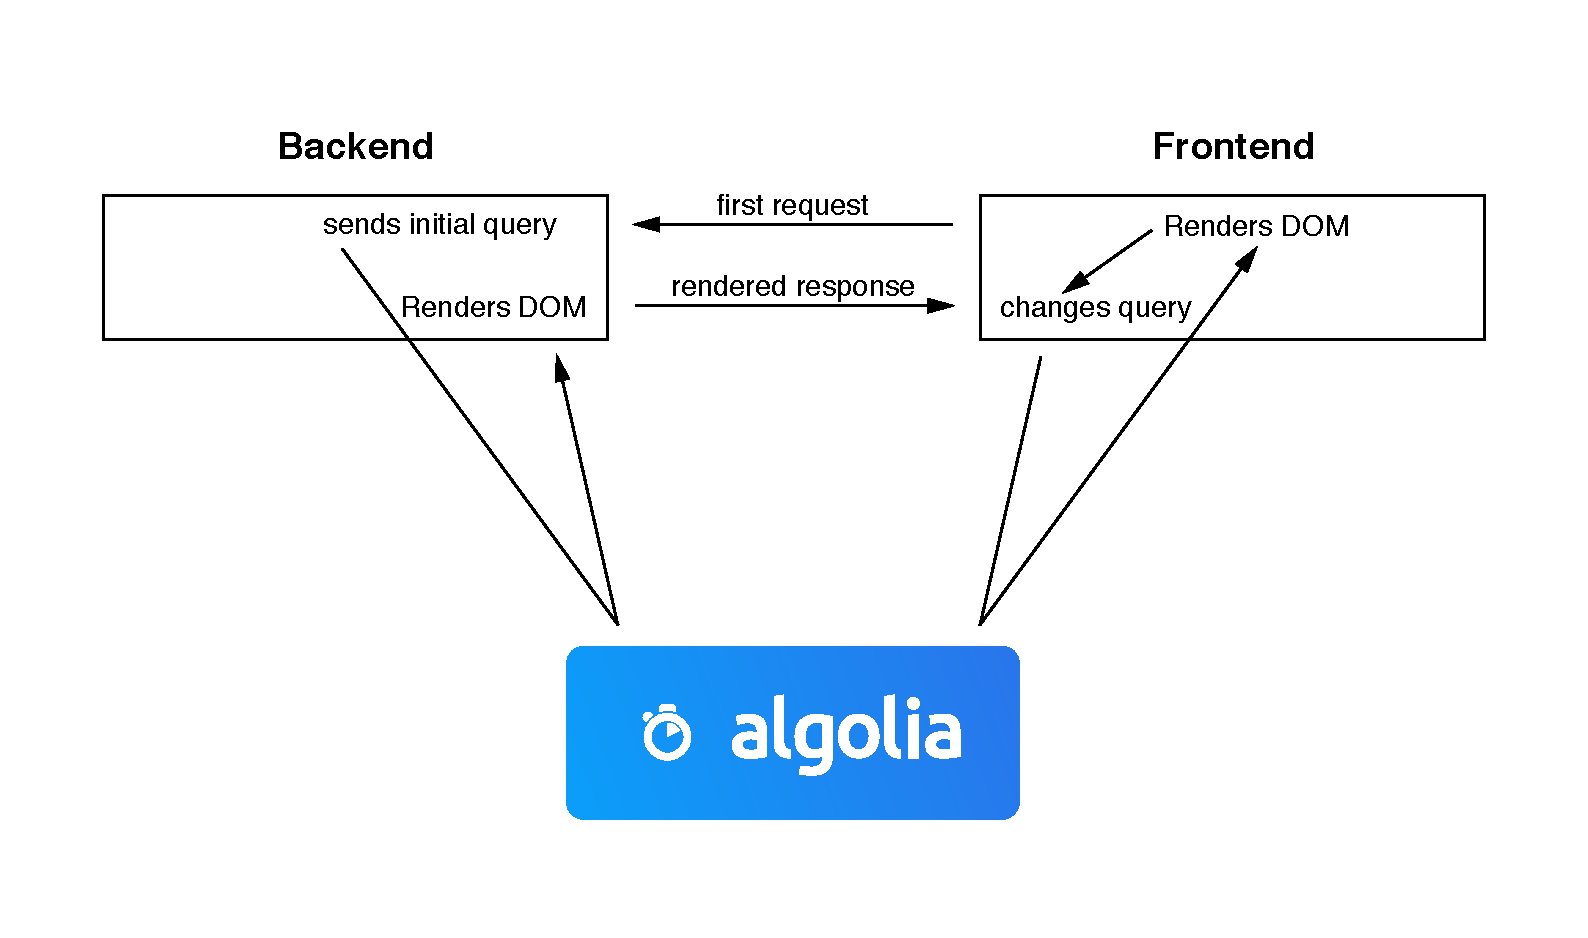
\includegraphics[width=0.6\textwidth, height=0.2\textheight, draft]{../assets/is-core-ssr.pdf}
  \caption{Server Side Rendering with InstantSearch Core}
  \label{figure:is-core-ssr}
\end{figure} %%

% section saved_state (end)

\section{Overview} % (fold)
\label{sec:overview}

\begin{figure}[H]
  \centering
  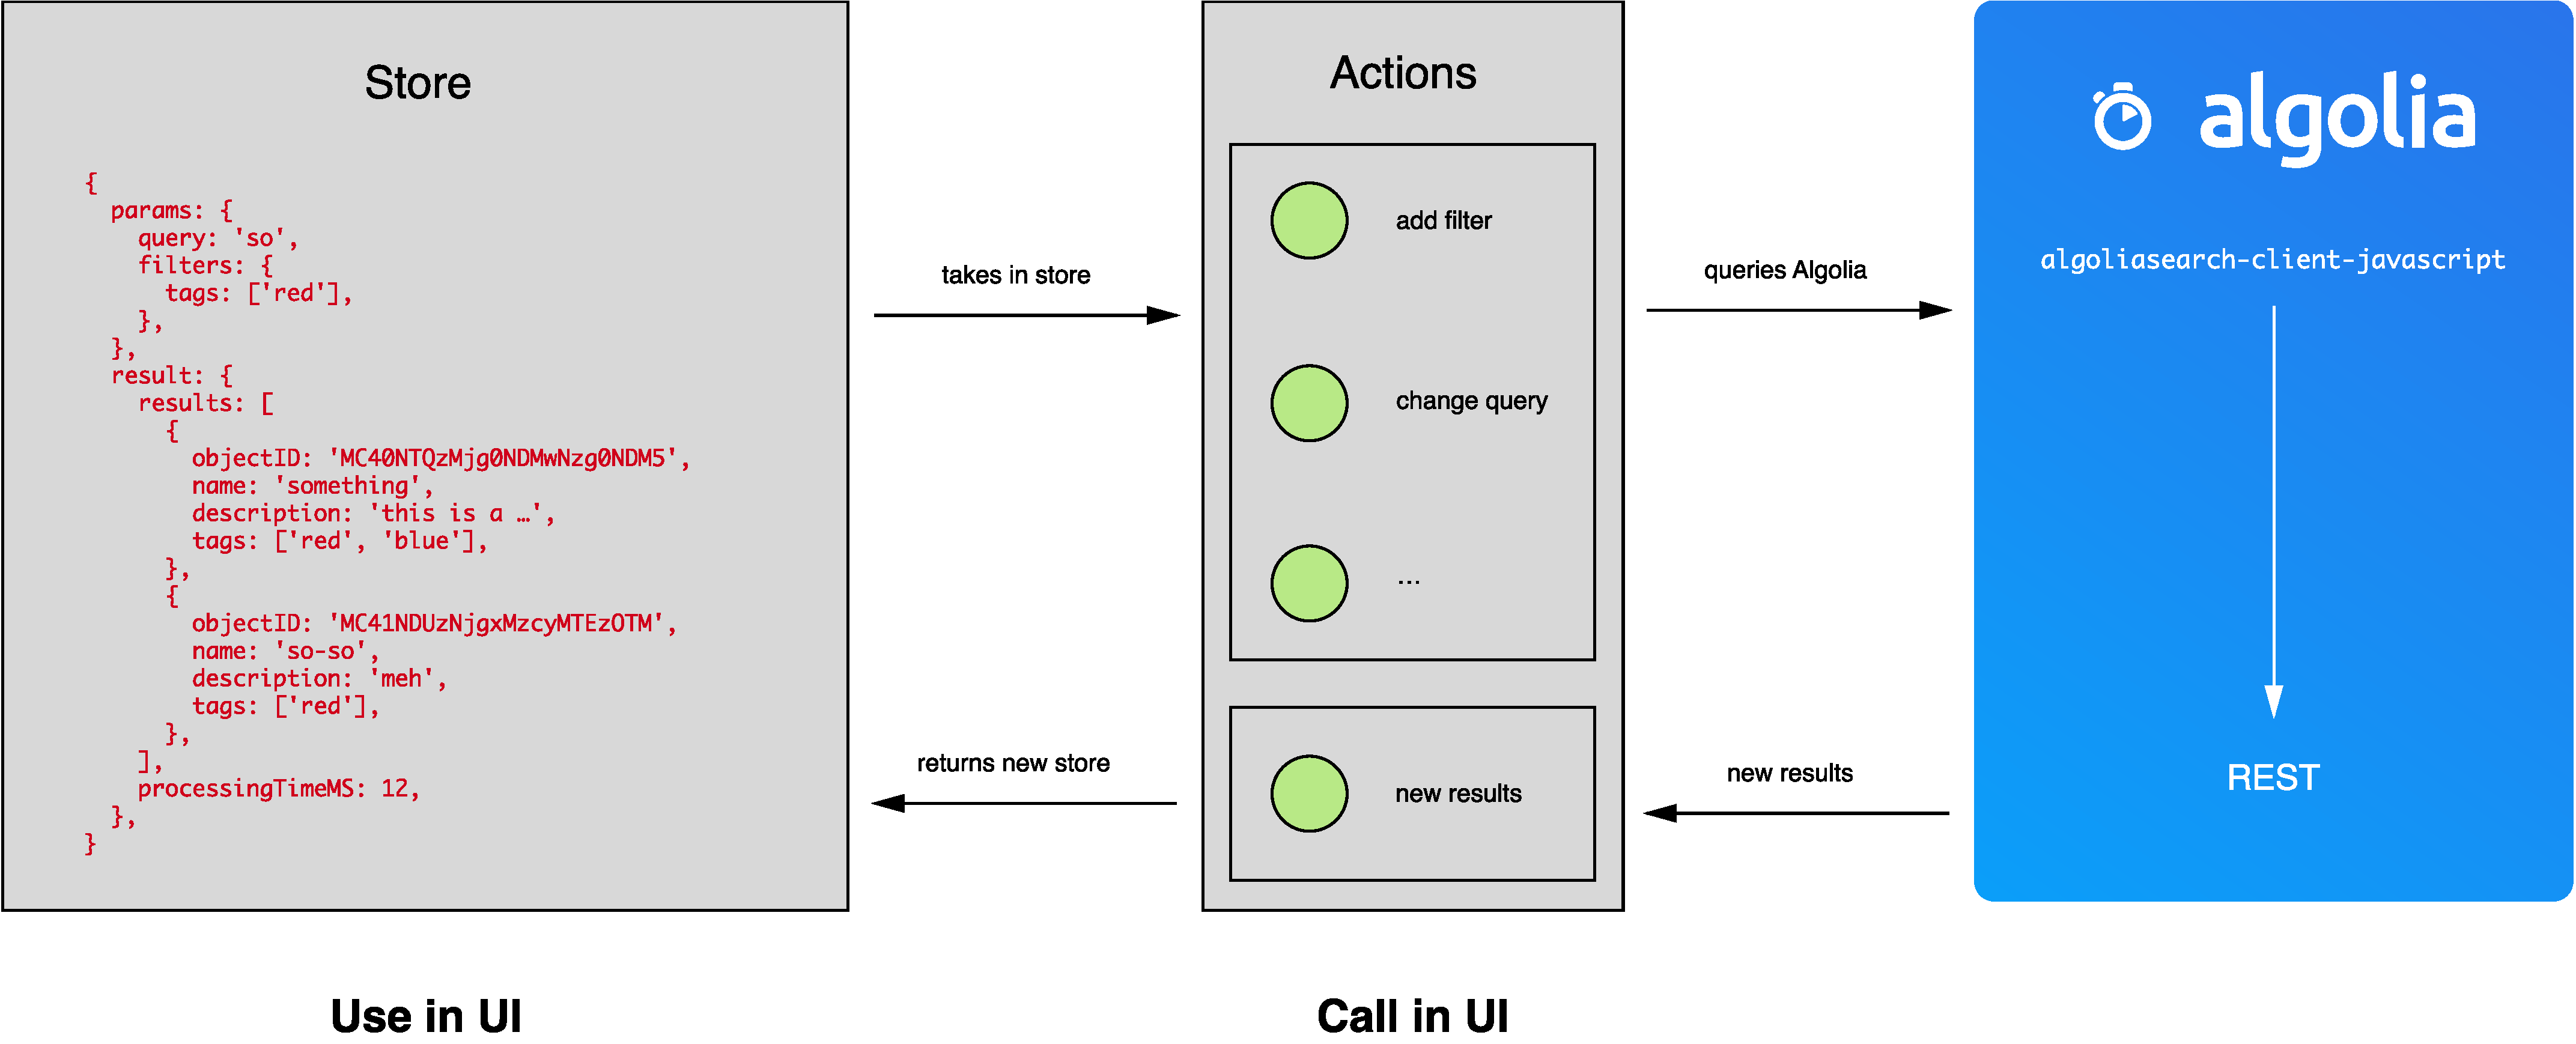
\includegraphics[width=\textwidth]{../assets/architecture.pdf}
  \caption{Architecture overview\cite{blog-architecture}}
  \label{figure:core-architecture}
\end{figure}

TODO: update this image with more recent architecture %%

% section overview (end)

\section{Usage in libraries} % (fold)
\label{sec:usage_in_libraries}

PoC in instantsearch.js and React InstantSearch for the RefinementList %%

% section usage_in_libraries (end)
